\begin{figure}[t]
	\centering
	\begin{subfigure}{0.33\linewidth}
		\includegraphics[width=1\linewidth]{plots/FitzNagNoNoise/TopLeft}
	\end{subfigure}
	\hspace*{.66\textwidth}\quad
	
	\begin{subfigure}{0.32\linewidth}
		\includegraphics[width=1\linewidth]{plots/FitzNagNoNoise/MiddleLeft}
	\end{subfigure}
	\begin{subfigure}{0.32\linewidth}
		\includegraphics[width=1\linewidth]{plots/FitzNagNoNoise/MiddleMiddle}
	\end{subfigure}
	\hspace*{.33\textwidth}\quad
	
	\begin{subfigure}{0.32\linewidth}
		\includegraphics[width=1\linewidth]{plots/FitzNagNoNoise/BottomLeft}
	\end{subfigure}
	\begin{subfigure}{0.32\linewidth}
		\includegraphics[width=1\linewidth]{plots/FitzNagNoNoise/BottomMiddle}
	\end{subfigure}
	\begin{subfigure}{0.32\linewidth}
		\includegraphics[width=1\linewidth]{plots/FitzNagNoNoise/BottomRight}
	\end{subfigure}
	\caption{Marginal distributions for $\theta$ obtained with the deterministic solver. The posterior distributions are clearly concentrated and mutually singular.}
	\label{fig:FitzNagDet}
\end{figure}

\begin{figure}[t]
	\centering
	\begin{subfigure}{0.33\linewidth}
		\includegraphics[width=1\linewidth]{plots/FitzNagNoise/TopLeft}
	\end{subfigure}
	\hspace*{.66\textwidth}\quad
	
	\begin{subfigure}{0.32\linewidth}
		\includegraphics[width=1\linewidth]{plots/FitzNagNoise/MiddleLeft}
	\end{subfigure}
	\begin{subfigure}{0.32\linewidth}
		\includegraphics[width=1\linewidth]{plots/FitzNagNoise/MiddleMiddle}
	\end{subfigure}
	\hspace*{.33\textwidth}\quad
	
	\begin{subfigure}{0.32\linewidth}
		\includegraphics[width=1\linewidth]{plots/FitzNagNoise/BottomLeft}
	\end{subfigure}
	\begin{subfigure}{0.32\linewidth}
		\includegraphics[width=1\linewidth]{plots/FitzNagNoise/BottomMiddle}
	\end{subfigure}
	\begin{subfigure}{0.32\linewidth}
		\includegraphics[width=1\linewidth]{plots/FitzNagNoise/BottomRight}
	\end{subfigure}
	\caption{Marginal distributions for $\theta$ obtained with the probabilistic solver. The posterior distributions account for the numerical error.}
	\label{fig:FitzNagProb}
\end{figure}